\section{Part 1: Configuration of fieldbus using Syscon}
\subsection{Preparations}
The PC is connected by a CAT-5 ethernet cable to a FI302 unit in the field, consisting of power supply (PS302), terminator (PSI302) and processor (FI302).

\subsection{Communication}
The network is terminated in both ends, and BT is connected to OUT+. 

The network is now powered, but does not have any nodes/units connected. In this assignment we will first do the physical set-up, before we do the logic.


\subsection{Syscon Start-up}
Syscon started, and file created with the name \textbf{Gruppe 05.}

\subsection{Adding network and initializing communication}

\textbf{myBus} created as $\textbf{New Fieldbus...}$ with the following \textbf{Communication Settings:}

\textbf{- Server ID:} Smar.DFIOLEServer.0

\textbf{- Server Context:} All.

\textbf{- Node Name:} myBus

$\rightarrow$ Communication initialized.

\newpage
\subsection{Adding new bridge for ethernet/fieldbus}
\textbf{New bridge} created.

\begin{figure}[!htb]
    \centering
    \centerline{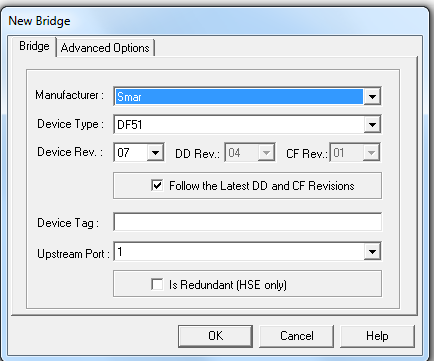
\includegraphics[width=0.5\textwidth]{images/newBridge}}
    \caption{New bridge}
    \end{figure}


Commissioning of the new bridge was applied to check the \textbf{Device Configuration} against the \textbf{Physical Device}.

\textbf{Device Configuration}:

Device Rev. $\rightarrow$ 07

DD Rev. $\rightarrow$ 04

CF Rev. $\rightarrow$ 01

\textbf{Physical Device}:

Device Rev. $\rightarrow$ 07

DD Rev. $\rightarrow$ 01

CF Rev. $\rightarrow$ 01

\begin{figure}[!htb]
    \centering
    \centerline{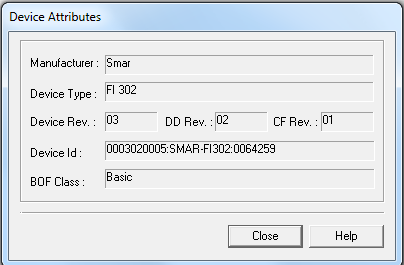
\includegraphics[width=0.5\textwidth]{images/DeviceAttributesFI302}}
    \caption{Device Attributes FI302}
    \end{figure}

\begin{figure}[!htb]
    \centering
    \centerline{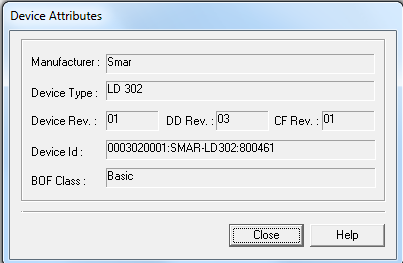
\includegraphics[width=0.5\textwidth]{images/DeviceAttributesLD302}}
    \caption{Device Attributes LD302}
    \end{figure}
    


The \textbf{Exchange} function was used to apply the \textbf{Physical Device Rev}. for both (07, 01, 01).

The Rev. values from the \textbf{Livelist} was noted for further tasks.

\begin{figure}[!htb]
    \centering
    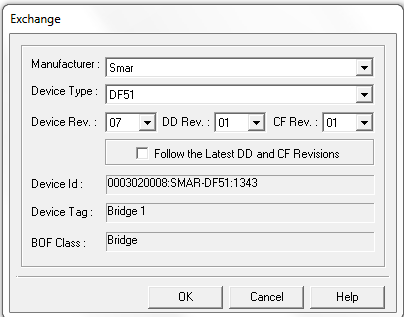
\includegraphics[width=0.5\textwidth]{images/ChangeofRev}
    \caption{Exchange}
    \end{figure}

\newpage
\subsection{FI302 and LD302}
FI302 and LD302 were added as \textbf{New Device} with the same Rev. values found in the Livelist. Then we used \textbf{Commission} to establish contact with the nodes. 

\begin{figure}[!htb]
    \centering
    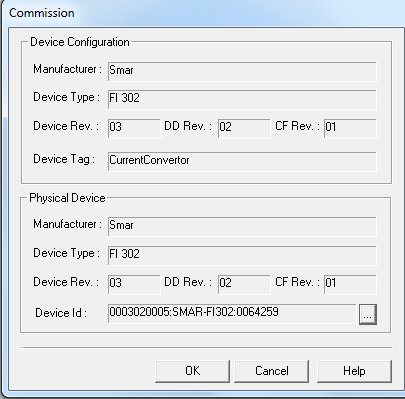
\includegraphics[width=0.5\textwidth]{images/ComissionFI}
    \caption{Commission FI}
    \end{figure}
    
\begin{figure}[!htb]
    \centering
    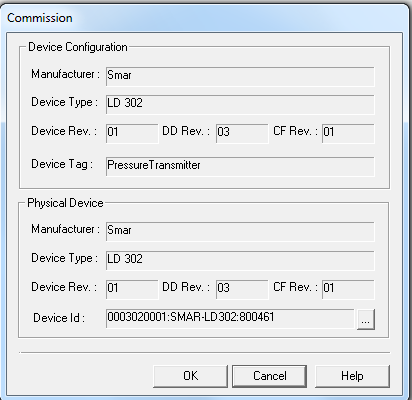
\includegraphics[width=0.5\textwidth]{images/CommissionLD}
    \caption{Commission LD}
    \end{figure}

\newpage
\subsection{Implementing function blocks for the field units}
\textbf{Transducer block:} Insulates the function block from the specific I/O hardware, such as sensors, actuators. Transducer block controls access to I/O through manufacturer specific implementation. This permits the transducer block to execute as frequently as necessary to obtain good data from sensors without burdening the function blocks that use the data. It also insulates the function block from the manufacturer specific characteristics of certain hardware. By accessing the hardware, the transducer block can get data from I/O or passing control data to it. The connection between Transducer block and Function block is called channel. These blocks can exchange data from its interface.
Normally, transducer blocks perform functions, such as linearization, characterization, temperature compensation, control and exchange data to hardware.

\textbf{Resource block:} Are used to define hardware specific characteristics of function block applications. Similar to transducer blocks, they insulate function blocks from the physical hardware by containing a set of implementation independent hardware parameters.


    
    

We added the function blocks as:

\textbf{AI} $\rightarrow$ Pressure Transmitter.
 
\textbf{AO} $\rightarrow$ Current Converter.

\subsection{Function block parameters}
\textbf{MODE\_BLK:} has 4 elements.
\begin{itemize}
    \item {Target - This is the mode requested by the operator. Only one mode from those allowed by the permitted mode parameter may be requested, that check will be done by the device.}
    \item {Actual - This is the current mode of the block, which may differ from the target based on operating conditions and block configuration, as input parameter status and bypass configuration, for example. Its value is always calculated as part of block execution, therefore the user can not write in this attribute.}
    \item {Permitted – It defines the modes that are allowed for an instance of the block. The permitted mode is configured based on the application requirement. For example, if a PID block does not have link for CAS\_IN, the Cas mode should not be permitted for that block. It is like a list of mode types selected from the supported modes.}
    \item{Normal - This is the mode which the block should be set to during normal operating conditions. The normal attribute is used as a reminder. It does not affect the algorithm calculation.}
   
 \end{itemize}

\textbf{XD\_SCALE}: The AI block has the XD\_SCALE parameter to define the engineering units expected from the transducer.

\textbf{OUT\_SCALE}: When the OUT value exceeds the OUT\_SCALE range and no worse condition exists in the block then the OUT status will be "uncertain, EU Range Violation".

\textbf{PV\_SCALE}: Converts the error to percentage (PID).

\textbf{L\_TYPE}: The L\_TYPE parameter determines how the values passed by the transducer block will be used into the block. The options are:
\begin{itemize}
    \item{Direct - the transducer value is passed directly to the PV. Therefore OUT\_SCALE is useless.}
    \item{Indirect - the PV value is the FIELD\_VAL value converted to the OUT\_SCALE.}
    \item{Indirect with Square Root} - the PV value is square root of the FIELD\_VAL converted to the OUT\_SCALE.
} 
\end{itemize}

\textbf{CHANNEL}: The CHANNEL parameter configuration depends on the device features as it follows:
\begin{itemize}
    \item{Fixed I/O Device: This type of device has a fixed number of I/O. All Smar field devices belong to this class. The channel is numbered from 1 to the maximum number of I/O.}
    \item{Configurable I/O Device: The user may configure the number of I/O modules as well the I/O type (input, output, discrete, analog, pulse,...). The DFI302 is the only device classified as a configurable I/O decice. All I/O modules have the I/O points arranged as Point (P), Group (G), Slot (S) and Rack (R).}
} 
\end{itemize}

\textbf{TERMINAL\_NUMBER}: Is used to assign inputs to belonging transducer.
